% $Id$
% ---------------------------------------------------------------------------
%
%  This is part of the SIGI.
%  Copyright (C) 2008 Interlegis
%  See the file relatorio.tex for copying conditions.
%

\section{Casos de Uso}
\label{sec:casos}

Esta seção descreve a utilização do sistema através de \emph{Casos de
  Uso}, representando os principais atores e suas interações com o
sistema.

Os Casos de Uso servem de auxílio à compreensão dos usuários quanto à
implementação e uso do sistema.

\subsection{Casos de Uso do SIGI}
A Figura \ref{fig:casos} apresenta os Casos de Uso do SIGI de maneira
simplificada.

\begin{figure}[h]
  \centering
  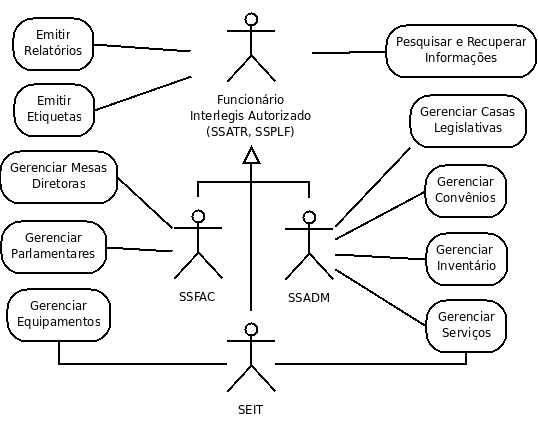
\includegraphics[width=120mm]{../imagens/casosdeuso.png}
  \caption{Casos de Uso}
  \label{fig:casos}
\end{figure}

\subsubsection{Descrição dos Atores}
\begin{description}
\item[Funcionário Interlegis Autorizado:] usuário apenas com
  atribuições de leitura no sistema. Inclui pessoal da Subsecretaria
  de Apoio Técnico e Relações Institucionais (SSATR) e Subsecretaria
  de Planejamento e Fomento (SSPLF).
\item[SSFAC:] Subsecretaria de Formação e Atendimento à Comunidade do
  Legislativo.
\item[SSADM:] Subsecretaria de Administração.
\item[SEIT:] Serviço de Infra-estrutura Tecnológica.
\end{description}

\subsubsection{Descrição das Atividades}
\begin{description}
\item[Emitir Relatórios:] consiste em obter informações e emitir
  relatórios de diversas partes do sistema.
\item[Emitir Etiquetas:] consiste em obter informações e emitir
  etiquetas de algumas partes do sistema.
\item[Pesquisar e Recuperar Informações:] habilidades de pesquisa e
  obtenção de informações da base de dados do sistema.
\item[Gerenciar Mesas Diretoras:] consiste em inserir, atualizar e
  remover \emph{Mesas Diretoras}, \emph{Sessões Legislativas} e
  modificar a \emph{Composição das Mesas Diretoras}.
\item[Gerenciar Parlamentares:] consiste em inserir, atualizar e
  remover \emph{Parlamentares} e \emph{Partidos}.
\item[Gerenciar Equipamentos:] consiste em inserir, atualizar e
  remover \emph{Equipamentos} e \emph{Fornecedores}.
\item[Gerenciar Casas Legislativas:] consiste em inserir, atualizar e
  remover \emph{Casas Legislativas}.
\item[Gerenciar Convênios:] consiste em inserir, atualizar e remover
  \emph{Convênios}.
\item[Gerenciar Inventário:] consiste em atualizar o \emph{Inventário}
  das Casas Legislativas.
\item[Gerenciar Serviços:] consiste em inserir, atualizar e remover
  \emph{Serviços} prestados às Casas Legislativas.
\end{description}

%
% Local variables:
%   mode: flyspell
%   TeX-master: "relatorio.tex"
% End:
%
